\documentclass[border=14pt]{standalone}
\usepackage[T1]{fontenc}
\usepackage{lmodern}
\usepackage{amsmath}
\usepackage{tikz}
\usetikzlibrary{positioning, arrows.meta, fit, backgrounds}

\definecolor{inputfill}{HTML}{EDF2F7}
\definecolor{inputline}{HTML}{7D8CA3}
\definecolor{blockfill}{HTML}{DCE6F2}
\definecolor{blockline}{HTML}{4A6285}
\definecolor{outfill}{HTML}{F3E8DC}
\definecolor{outline}{HTML}{A8784A}
\definecolor{panelfill}{HTML}{FAFAFA}
\definecolor{panelline}{HTML}{C9CFD8}

\begin{document}
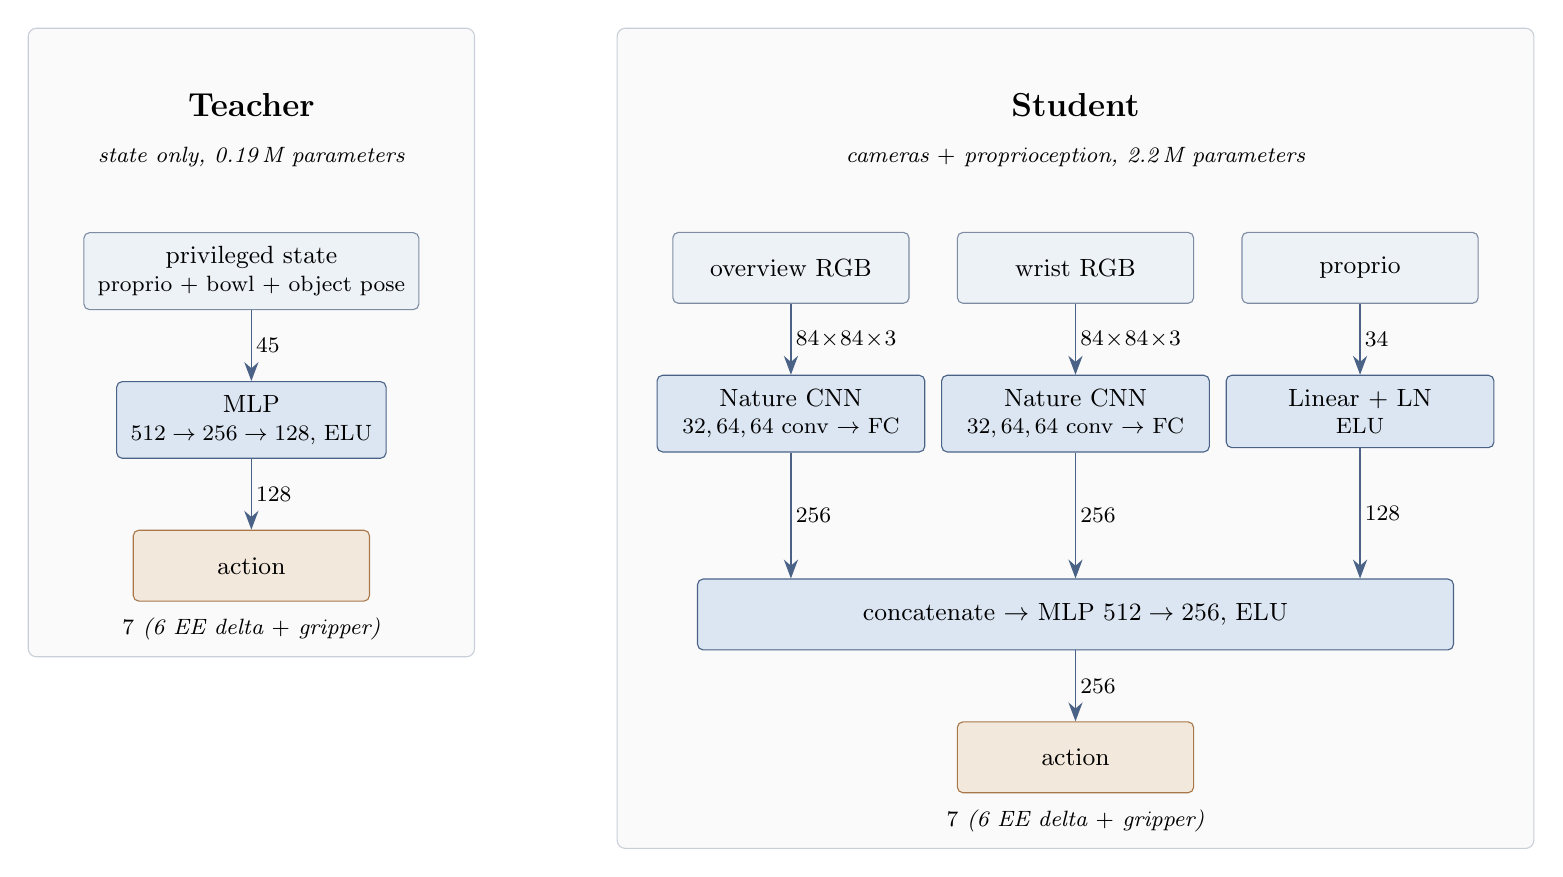
\begin{tikzpicture}[
  font=\small,
  node distance=9mm,
  box/.style   = {rounded corners=2pt, draw, align=center, inner sep=5pt, minimum height=9mm},
  input/.style = {box, fill=inputfill, draw=inputline, minimum width=30mm},
  block/.style = {box, fill=blockfill, draw=blockline, minimum width=34mm},
  outbox/.style = {box, fill=outfill,   draw=outline,   minimum width=30mm},
  flow/.style  = {-{Stealth[length=2.4mm]}, draw=blockline, line width=0.5pt},
  dim/.style   = {font=\footnotesize\itshape, inner sep=1.5pt},
  title/.style = {font=\large\bfseries},
  sub/.style   = {font=\footnotesize\itshape},
]

%% ---------------------------------------------------------------- teacher
\node[title] (ttitle) {Teacher};
\node[sub, below=1.5mm of ttitle] (tsub) {state only, 0.19\,M parameters};

\node[input, below=7mm of tsub] (tin) {privileged state\\[-1pt]\footnotesize proprio $+$ bowl $+$ object pose};
\node[block, below=of tin]       (tmlp) {MLP\\[-1pt]\footnotesize $512 \to 256 \to 128$, ELU};
\node[outbox,   below=of tmlp]      (tout) {action};

\draw[flow] (tin)  -- node[dim, right] {$45$} (tmlp);
\draw[flow] (tmlp) -- node[dim, right] {$128$} (tout);
\node[dim, below=1.5mm of tout] {$7$ (6 EE delta $+$ gripper)};

%% ---------------------------------------------------------------- student
\node[title, right=86mm of ttitle] (stitle) {Student};
\node[sub, below=1.5mm of stitle] (ssub) {cameras $+$ proprioception, 2.2\,M parameters};

\node[input, below=7mm of ssub]   (scam2) {wrist RGB};
\node[input, left=6mm of scam2]   (scam1) {overview RGB};
\node[input, right=6mm of scam2]  (sprop) {proprio};

\node[block, below=of scam1] (senc1) {Nature CNN\\[-1pt]\footnotesize $32,64,64$ conv $\to$ FC};
\node[block, below=of scam2] (senc2) {Nature CNN\\[-1pt]\footnotesize $32,64,64$ conv $\to$ FC};
\node[block, below=of sprop] (senc3) {Linear $+$ LN\\[-1pt]\footnotesize ELU};

\node[block, below=16mm of senc2, minimum width=96mm] (sfuse) {concatenate $\to$ MLP $512 \to 256$, ELU};
\node[outbox,   below=of sfuse] (sout) {action};

\draw[flow] (scam1) -- node[dim, right] {$84\!\times\!84\!\times\!3$} (senc1);
\draw[flow] (scam2) -- node[dim, right] {$84\!\times\!84\!\times\!3$} (senc2);
\draw[flow] (sprop) -- node[dim, right] {$34$} (senc3);
\draw[flow] (senc1) -- node[dim, right] {$256$} (senc1 |- sfuse.north);
\draw[flow] (senc2) -- node[dim, right] {$256$} (senc2 |- sfuse.north);
\draw[flow] (senc3) -- node[dim, right] {$128$} (senc3 |- sfuse.north);
\draw[flow] (sfuse) -- node[dim, right] {$256$} (sout);
\node[dim, below=1.5mm of sout] {$7$ (6 EE delta $+$ gripper)};

%% ---------------------------------------------------------------- panels
\begin{scope}[on background layer]
  \node[draw=panelline, fill=panelfill, rounded corners=3pt, inner sep=7mm,
        fit=(ttitle)(tin)(tout)] {};
  \node[draw=panelline, fill=panelfill, rounded corners=3pt, inner sep=7mm,
        fit=(stitle)(scam1)(sprop)(sout)] {};
\end{scope}
\end{tikzpicture}
\end{document}
